\documentclass [12pt]{report}
\usepackage{times}
\usepackage[nohead,left=3cm,right=3cm,bottom=3.5cm,top=3.5cm,a4paper]{geometry}
\usepackage{graphicx}
\usepackage{subcaption}
\usepackage[english]{babel}
%\usepackage[onehalfspacing]{setspace}
\usepackage{hyperref}
\usepackage{amsmath}
\usepackage{bm}
\usepackage{algpseudocode}
\usepackage{algorithm}
\usepackage[nottoc]{tocbibind}
\usepackage{appendix}
\usepackage{scrextend}
\usepackage{caption}
\captionsetup{labelfont=bf, format=hang, labelsep=period}

\exhyphenpenalty=1000
\hyphenpenalty=1000
\linespread{1.15}

\title{Calculating the Zero Point Energy of Ethane Using the Diffusion Quantum Monte Carlo Method}
\author{Simon Neidhart \\ \\ Supervisor: Prof. Dr. Stefan Goedecker}
\date{University of Basel \\ \today}



\begin{document}
\maketitle
\tableofcontents
\newpage
\chapter{Introduction}
Monte Carlo methods are almost as old as computers. Its first application was to simulate neutron transport in fissionable material. Here, the outcome of collisions with the material as well as the different types of collisions or reactions are the random parts of the problem and thus require random numbers to simulate in a computer. This simulation is very intuitive as the computer simulates directly what happens in nature. The mathematical reason that this works, is that the underlying integral is in fact solved by numerical integration using these random numbers. Once people realized this, the application of Monte Carlo methods started to drift away from the obvious problems such as fission and more towards any problem that needs to solve a high dimensional integral. It is very important to keep this mathematical foundation in mind as the most intuitive approaches are often not the most efficient to do a Monte Carlo calculation.\\
Inspired by this, we exploit the similarity between the Schrödinger equation and the diffusion equation to develop the Diffusion Quantum Monte Carlo (DQMC) algorithm. It is rather obvious where the the randomness lies in pure diffusion and a short derivation will show that this can also be applied to solving the many-body Schrödinger equation. In the field of quantum mechanics, Monte Carlo simulations can be very useful as there are a lot of high dimensional integrals that need to be solved. Of the many approaches that exist in quantum Monte Carlo, DQMC is the most versatile.\\
In this work, the aim is to calculate zero point energies with the developed DQMC algorithm. In the first step, the algorithm is tested using the well known quantum harmonic oscillator. Then, it is applied to the molecule of ethane to calculate its zero point energy. The result is then compared to a reference calculation and we conclude that the algorithm performed very well.

\chapter{Theoretical Background}
This chapter covers the derivation and the theory behind the developed DQMC algorithm from a mathematical and physical standpoint. It aims to act as a guide to anyone who wants to understand the theory behind the algorithm or implement the algorithm.

\section{The Born-Oppenheimer Approximation}
When considering a system of $N_{at}$ nuclei with positions $\bm{R}_i,...,\bm{R}_{N_{at}}$, masses $m_1,...,m_{N_{at}}$ and charge numbers $Z_1,...,N_{N_{at}}$ and $N$ electrons with positions $\bm{r}_i,...,\bm{r}_{N_{at}}$, the Born-Oppenheimer approximation justifies splitting the problem (and therefore also the Hamiltonian into two separate problems. First, the electronic part of the Hamiltonian
\begin{equation}
\mathcal{H}^e = - \frac{1}{2}\sum_{i=1}^N \nabla^2_{\bm{r}_i}  + \sum_{i=1}^{N} \sum_{j=1}^{i-1} \frac{1}{|\bm{r}_i-\bm{r}_j|} - \sum_{i=1}^{N} \sum_{j=1}^{N_{at}} \frac{Z_j}{|\bm{r}_i-\bm{R}_j|} + \sum_{i=1}^{N_{at}} \sum_{j=1}^{i-1} \frac{Z_i Z_j}{|\bm{R}_i-\bm{R}_j|}
\end{equation}
containing the kinetic term of the electrons, the electron-electron, electron-nuclei and nuclei-nuclei interactions, is solved. In this work, we will use existing electronic structure codes to solve the electronic Schrödinger equation. This gives a potential energy surface (PES) $E_0^e(\bm{R}_i,...,\bm{R}_{N_{at}})$ with a minimum $E_{min}^e$. Since we do not have to worry about the electrons anymore, we will from now on write all atom coordinates in one vectctor $\bm{x} = \bm{R}_i,...,\bm{R}_{N_{at}}$ of length $3N_{at}$.
The second part of the problem is the nucleonic Schrödinger equation
\begin{equation} \label{eq:2.2}
\sum_{i=1}^{N_{at}} \frac{-1}{2m_i} \nabla^2_{\bm{R_i}} \psi^n + E_0^e \psi^n = \mathcal{H} \psi^n = E_0 \psi^n,
\end{equation}
which we will solve for the energy $E_0$ using the DQMC algorithm. The Born-Oppenheimer approximation is justified by the fact that the nuclei are much heavier than the electrons and can therefore be treated classically in the electronic structure problem but then quantum-mechanically in the nucleonic Schrödinger equation. From the point of view of the electrons, the nuclei are basically stationary and therefore, their slow movement does not influence the solution of the electronic structure problem. The nuclei then feel the potential from the electrons and move accordingly on the PES.
In this work, the goal is to calculate the zero-point energy (ZPE) of a system of atoms. The ZPE is defined as the difference between $E_{min}^e$ and $E_0$. Because the kinetic energy (first term in eq. \eqref{eq:2.2}) is always positive, $E_0$ is always greater than $E_{min}^e$ and therefore the ZPE is always positive.

\section{Monte Carlo Methods}
%evtl löschen
The core of the Monte Carlo approach is to do numerical calculations by using lots of random numbers distributed according to a desired probability distribution $p(x)$ to approximate expectation values or integrals with averages over many trials.
\begin{equation}
\langle \mathcal{A} \rangle = \sum_{x \in \Omega} \mathcal{A}(x) p(x) \approx \frac{1}{N} \sum_{i=1}^N \mathcal{A}(x_i),
\end{equation}
or
\begin{equation}
\int_{x \in \Omega} \mathcal{A}(x) p(x) d^n x \approx \frac{1}{N} \sum_{i=1}^N \mathcal{A}(x_i),
\end{equation}
where $x_i$ are the random numbers generated according to the probability distribution $p(x)$. Because doing a sum or integral over the entire space $\Omega$ is often not possible because the space is too large, one generates the $x_i$ from a Markov Chain. This means that from a given $x_i$, $x_{i+1} = f(x_i,i,$"noise"$)$ can be generated using a stochastic process. To ensure that the $x_i$ follow the probability distribution $p(x)$ a acceptance-rejection step needs to be introduced. Namely, if $\alpha = \frac{p(x_{i+1})}{p(x_i)} > 1$ the new value $x_{i+1}$ always gets accepted and if $\alpha < 1$ the new value $x_{i+1}$ only gets accepted with probability $\alpha$. Put together, these steps leads to the Metropolis algorithm (Appendix \ref{appendixB}). These ingredients form the basis of most Monte Carlo methods including the here presented DQMC algorithm.
\section{Diffusion Quantum Monte Carlo}
To get the ZPE, we now solve the nucleonic Schrödinger equation \eqref{eq:2.2} for the energy $E_0$ using diffusion quantum Monte Carlo. There are two main ways to derive the DQMC algorithm but the most common one is by a transformation to of the Schrödinger equation to an imaginary time $\tau = it$ \cite{mccoy,cyrus,herleitung2}. The Schrödinger equation then becomes
\begin{equation} \label{eq:2.5}
\frac{\partial}{\partial \tau} \psi(\bm{x},\tau) = -(\mathcal{H} - E_T) \psi(\bm{x},\tau),
\end{equation}
where the energy is shifted by the trial energy $E_T$. The wave function can now be written as
\begin{equation} \label{eq:2.6}
\psi(\bm{x},\tau) = \sum_{i=1}^{\infty} e^{-(E_i - E_T)\tau}\psi_i(\bm{x}),
\end{equation}
where $E_i$ and $\psi_i(\bm{x})$ solve the time independent nucleonic Schrödinger equation $\mathcal{H}\psi_i(\bm{x}) = E_i \psi_i(\bm{x})$ and $E_0 \leq E_1 \leq E_2 \leq...$.
As we now increase our simulation time $\tau$, the sum only converges to the ground state wave function $\psi_0(\bm{x})$ if we adjust $E_T$ to $E_0$ as all other terms decay exponentially faster. This happens independent of the inital choice of our wave function.
As we now discretize our time step, we get the known short time propagator of \eqref{eq:2.5} for moving a particle form position $\bm{x}$ to position $\bm{y}$ during a short time step $\Delta \tau$
\begin{equation} \label{eq:2.7}
G(\bm{x_i},\bm{y}_i;\Delta \tau) = \sqrt{\frac{m_i}{2 \pi \Delta \tau}} e^{-(\bm{x}_i-\bm{y}_i)^2 m_i/(2 \Delta \tau)} e^{-\Delta t (E_0(\bm{y}) - E_T)} + \mathcal{O}(\Delta \tau^2),
\end{equation}
for $i=1,...,3N_{at}$. This propagator has two parts. The first part $\sqrt{\frac{m_i}{2 \pi \Delta \tau}} e^{-(\bm{x}_i-\bm{y}_i)^2 m_i/(2\Delta \tau)}$ is pure diffusion for dimension $i$ and corresponds to a Gaussian distribution centered around $\bm{x}_i$ giving a smaller value, the further $\bm{y}_i$ is away from $\bm{x}_i$. The second part $q = e^{-\Delta \tau (E_0^e(\bm{y}) - E_T)}$ represents a branching process. If $E_0^e(\bm{y}) > E_T$ then $q < 1$ and if $E_0^e(\bm{y}) < E_T$ then $q > 1$.\\
Up to this point, we have derived the unguided DQMC algorithm. To improve the convergence it is very useful to introduce a trial or guiding wave function $\psi_T(\bm{x})$. $\psi_T$ should approximate $\psi(\bm{x})$ as good as possible, without requiring to much effort to compute and evaluate. Our program will later need a lot of evaluations of the first and second derivative of $\psi_T(\bm{x})$. We now multiply the Schrödinger equation \eqref{eq:2.5} with $\psi_T(\bm{x})$, define $f(\bm{x}) = \psi(\bm{x}) \psi_T(\bm{x})$ and after some calculation \cite{cyrus2} we get
\begin{equation} \label{eq:2.8}
\sum_{i=1}^{N_{at}} \frac{-1}{2m_i} \nabla^2_{\bm{R}_i} f(\bm{x}) + \nabla_{\bm{x}} (\bm{v}(\bm{x}) f(\bm{x})) + (E_L(\bm{x}) - E_T)f(\bm{x}) = 0.
\end{equation}
We have now introduced the drift velocity $\bm{v}(\bm{x}) = \nabla \psi_T(\bm{x})/ \psi_T(\bm{x})$ and the local energy 
\begin{equation}\label{el}
E_L(\bm{x}) = (H\psi_T(\bm{x}))/\psi_T(\bm{x}) = \sum_{i=1}^{N_{at}} \frac{-1}{2m_i} \nabla^2_{\bm{R}_i} \psi_T(\bm{x}) + E_0^e(\bm{x}),
\end{equation}
and similarly to the unguided case, we can get the short-time propagator
\begin{equation} \label{eq:2.9}
\tilde{G}(\bm{x_i},\bm{y}_i;\Delta \tau) = \sqrt{\frac{m_i}{2 \pi \Delta \tau}} e^{-(\bm{x}_i-\bm{y}_i-\bm{v}(\bm{x})\Delta \tau)^2 m_i/(2 \Delta \tau)} e^{-\Delta \tau (E_L(\bm{x})+E_L(\bm{y}))/2 - E_T)} + \mathcal{O}(\Delta \tau^2).
\end{equation}
There are two major differences compared to the unguided propagator. In addition to the pure diffusion described by the Gaussian distribution, we now have the drift velocity, which drifts $\bm{x}$ towards a region where $f(\bm{x})$ is large. Second, the local energy adds the kinetic energy of the nuclei to the evaluation of the PES and the local energy is averaged over the position before and after the propagation. 
With these ingredients we can construct our DQMC algorithm using a population of walkers and simulating diffusion on them. First, we just update the walker position according to the first part of the propagator by displacing it according to
\begin{equation}\label{eq:2.10}
\bm{y}_i = \bm{x}_i + \bm{\eta}_i + \bm{v}_i(\bm{x})\Delta \tau/m_i \quad \textrm{ for } \quad i=1,...,N_{at},
\end{equation}
where $\bm{\eta}$ is a vector of $N_{at}$ normal distributed random numbers with mean $0$ and standard deviation $\sqrt{\Delta \tau / m_i}$ for dimension $i$.
The branching process can be implemented by letting walkers die, survive or reproduce according to their weight $w$ which is updated from step $k$ to step $k+1$ according to 
\begin{equation}\label{eq:2.11} 
w^{(k+1)} = w^{(k)} e^{(-\Delta \tau (E_L(\bm{x}) + E_L(\bm{y}))/2 - E_T))}.
\end{equation}
With these non-integer weights, one can implement the split-join algorithm \cite{split_join} to do the branching process. There are many alternatives, but split-join has the advantage that it limits the duplication of walker that would occur with other methods.
 In each iteration the weight for each walker is updated according to \eqref{eq:2.11}. Walkers with a weight $w > 2$ split into $\lfloor w \rfloor$ walkers with new weights $w/\lfloor w \rfloor$. For two walkers $\alpha$ and $\beta$ with weight $w_\alpha < 1/2$ and $w_\beta < 1/2$ one keeps walker $\alpha$  with probability $w_\alpha/(w_\alpha + w_\beta)$ and walker $\beta$ otherwise. The surviving walker gets the new weight $(w_\alpha + w_\beta)$. All walkers with weight $1/2 \leq w \leq 2$ survive and keep their weight. This algorithm keeps the total weight of all walkers $W^{(k)} =  \sum_{i = 1}^{N_w^{(k)}} w_i^{(k)}$ constant during iteration $k$ and limits the duplication of walkers that would occur with the standard branching process.
 This process ensures that even walkers with a local energy higher than $E_T$ have a chance of surviving and therefore the entire PES is sampled if we run the simulation long enough. \\
The last step is to adjust the trial energy $E_T$. $E_T$ controls the population of walker and it therefore needs to be adjusted to keep the walker population from dying out or growing exponentially. Generally speaking, we need to decrease $E_T$ if the number of walkers is increasing and increase $E_T$ if the number of walkers is decreasing.  Like with the split-join algorithm, there are multiple ways to adjust the trial energy \cite{mccoy,alavi}. We will here use an approach \cite{cyrus} that makes use of the total weight $W^{(k)}$ after iteration $k$ and updates $E_T$ according to
\begin{equation}\label{eq:2.12} 
E_T^{(k+1)} = E_0^{(k)} + \xi \log(W^{(k)}/W^{(0)}),
\end{equation}
where $\xi > 0$ is a damping parameter, $W^{(0)}$ is the sum of weight at the start of the simulation and
\begin{equation}\label{eq:2.13} 
E_0^{(k)} = \frac{\sum_{i = 1}^{N_w^{(k)}} w_{i}^{(k)} E_L(\bm{x}_{i}^{(k)})}{\sum_{i = 1}^{N_w^{(k)}} w_{i}^{(k)} },
\end{equation}
is the current estimation of the ground state energy $E_0$. This artificial adjustment to the trial energy introduces the so called population-control error. This error is generally small and can be easily controlled as it decreases as $1/N_{walkers}$. At the end of the simulation, this estimate can be improved by averaging it over may iterations after the equilibration phase giving the final result of the calculation, the energy eigenvalue of the Schrödinger equation and, by subtracting $E^e_{min}$, also the ZPE. It makes sense to further average the ZPE over many identical runs to get even more accuracy. The statistical uncertainty of the ZPE is then defined as the standard deviation over $M$ identical runs \cite{herleitung2}
\begin{equation}
\Delta ZPE = \sqrt{\frac{1}{M} \sum_{i=1}^M(ZPE_i = \overline{ZPE})},
\end{equation}
where $\overline{ZPE}$ is the average of the ZPE over the $M$ runs.
\newpage
\section{The DQMC Algorithm}
Putting all this theory together, we get the guided DQMC algorithm.
\begin{algorithm}
\caption{Guided DQMC}\label{dqmc}
\begin{algorithmic}[1]
\Procedure{DQMC}{$steps, \Delta \tau, E_0^e(\bm{x}), \psi_T(\bm{x}), m$}
\State \textbf{initialize} $walkers$
\For{$i=1,steps$}
	\ForAll{$\bm{x}$ \textbf{in} $walkers$}
		\State \textbf{draw} $\bm{\eta} \sim \mathcal{N}(\bm{x},\sqrt{\Delta t/m})$
		\State $\bm{x} = \bm{x} + \bm{\eta} + \bm{v}(\bm{x})$ \Comment{Moving the walker}
		\State $w = w \: exp(-\Delta \tau (E_L(\bm{x})+E_L(\bm{x}_{prev}))/2 - E_T))$
		\If {($w > 2$)}
		\State \textbf{make} $\lfloor q \rfloor$ \textbf{copies of} $\bm{x}$ \textbf{with weight} $w/\lfloor w \rfloor$ \textbf{for the next cycle}
		\EndIf
		\If {($w < 1/2$)}
		\State \textbf{find another walker} $\bm{y}$ \textbf{with} $w_y < 1/2$
		\State \textbf{draw} $r \sim \mathcal{U}([0,1])$
		\If{($w/(w+w_y) > r)$)}
		\State \textbf{make a copy of} $\bm{x}$ \textbf{with weight} $w+w_y$ \textbf{for the next cycle}
		\Else
		\State \textbf{make a copy of} $\bm{y}$ \textbf{with weight} $w+w_y$ \textbf{for the next cycle}
		\EndIf
		\EndIf 
	\EndFor
	\State \textbf{update} $E_T$ \Comment{According to \eqref{eq:2.13}}
\EndFor 
\EndProcedure
\end{algorithmic}
\end{algorithm}
\newpage
\section{Gaussian Trial Wave Functions}
This section discusses a simple way of choosing a trial wave function that can be used for various molecular systems. The idea is to transform from the Cartesian coordinate system  to a coordinate system defined by the vibrational modes. In this coordinate system, we can use the harmonic approximation to calculate a Gaussian trial wave function that gives a good approximation of the exact trial wave function.\\
First, we need to calculate the Hessian matrix of the PES
\begin{equation}
H_{i,j} = \left. \frac{\partial^2 E_0^e(\bm{x})}{\partial \bm{x}_i \partial \bm{x}_j }\right|_{\bm{x} = \bm{x}^0},
\end{equation}
where $\bm{x}^0$ is the minimum energy configuration of the system. The Hessian matrix should be symmetric ($H_{i,j} = H_{j,i}$). Because it is calculated numerically it often is not exactly symmetric. It is therefore a good practice to symmetrize it by replacing it by $\frac{1}{2} H H^T$. It is also much faster and often more accurate to calculate the Hessian as the first derivative of the force vectors instead of the second derivative of the postilions. 
Then, we calculate the eigenvectors $\bm{u}^i$ and  eigenvalues $\lambda_i$
\begin{equation} \label{eigs}
H \bm{u}^i = \lambda_i \bm{u}^i = m_i \omega_i^2 \bm{u}^i,
\end{equation}
where $m_i$ is the mass and $\omega_i$ the frequency of the harmonic oscillation along the vibrational mode $\bm{u}^i$.\\
Because a translation or rotation of the entire molecule does not change the energy, six of the eigenvalues are zero for molecules with more than two atoms. This means that we now have $3 N_{at} - 6$ dimensions defined by the eigenvectors $\bm{u}^i$.\\
for the calculation of the local energy $E_L$ in equation \eqref{el} we need the masses for all the new $3 N_{at} - 6$ dimensions. To do this, we calculate the mass-scaled Hessian matrix
\begin{equation}
\tilde{H}_{i,j} = \left. \frac{1}{\sqrt{m_i m_j}}\frac{\partial^2 E_0^e(\bm{x})}{ \partial \bm{x}_i \partial \bm{x}_j }\right|_{\bm{x} = \bm{x}^0}.
\end{equation}
and its eigenvalues and eigenvectors
\begin{equation}
\tilde{H} \bm{\tilde{u}}^i = \tilde{\lambda}_i \bm{\tilde{u}}^i = \omega_i^2 \bm{\tilde{u}}^i.
\end{equation}
Comparing $\tilde{\lambda}_i \bm{u}^i = \omega_i^2 \bm{u}^i$ with $\lambda_i \bm{u}^i = m_i \omega_i^2 \bm{u}^i$ from \eqref{eigs}, we get $m_i = \lambda_i / \tilde{\lambda}_i$ for the masses of the $3 N_{at} - 6$ new dimensions.
From the eigenvalues of the Hessian matrix, we can now calculate the harmonic potential to approximate the PES
\begin{equation}
V(\bm{x}) = \frac{1}{2} \sum_{i=1}^{3N_{at}-6} \lambda_i \bm{x}_i^2 = \frac{1}{2} \sum_{i=1}^{3N_{at}-6} m_i \omega_i^2 \bm{x}_i^2.
\end{equation}
Note, that the vector $\bm{x}$ is now only of length $3 N_{at} - 6$ and  each element $\bm{x}_i$ describes the displacement from the minimum energy configuration along the normal mode $\bm{u}^i$.
We can also calculate the ground state energy in the harmonic approximation
\begin{equation}
E_0^{harm} = \frac{1}{2} \sum_{i=1}^{3N_{at}-6} \omega_i = \frac{1}{2}\sum_{i=1}^{3N_{at}-6}  \sqrt{\tilde{\lambda}_i} = \frac{1}{2} \sum_{i=1}^{3N_{at}-6}  \sqrt{\frac{\lambda_i}{m_i}}.
\end{equation}
This energy gives a good starting value for the trial energy $E_T$ at the beginning of the calculation. Finally we get the Gaussian trial wave function
\begin{equation}
\psi_T(\bm{x}) = \prod_{i=1}^{3N_{at}-6} \mathcal{N} e^{-\frac{1}{2} m_i \omega_i (\bm{x}_i - \bm{x}^0_i)^2} = \prod_{i=1}^{3N_{at}-6} \mathcal{N} e^{-\frac{1}{2} \frac{(\bm{x}_i - \bm{x}^0_i)^2}{\sigma_i^2}},
\end{equation}
where $\sigma_i^2 = 1/(m_i \omega_i) = 1/(m_i\sqrt{\tilde{\lambda}}_i)$. The big advantage of Gaussian trial wave functions is that the first and second derivatives can be calculated analytically. This gives
\begin{equation}
\bm{v}_i(\bm{x}) = \nabla_{\bm{x}_i} \psi_T(\bm{x})/ \psi_T(\bm{x}) = \frac{-(\bm{x}_i - \bm{x}^0_i)}{\sigma_i^2}
\end{equation}
for the drift velocity and 
\begin{equation}\label{el}
E_L(\bm{x}) = (H\psi_T(\bm{x}))/\psi_T(\bm{x}) = \sum_{i=1}^{N_{at}} \frac{-1}{2m_i \sigma^2_i} \left( \frac{(\bm{x}_i - \bm{x}^0_i)^2}{\sigma^2_i} - 1 \right) + E_0^e(\bm{x})
\end{equation}
for the local energy.
Gaussian trial wave functions only work well if the harmonic approximation is good. To check that, one can compare the PES with the harmonic approximation $V(x)$ for each dimension. The harmonic approximation should match the true PES a bit beyond the energy $E_0^{harm}$ as good as possible to get fast and accurate results.
\section{Implementation Details and Improvements}
\subsection{Energy Calculations}
To evaluate the potential energy surface in the calculation of $E_L(\bm{x})$, we use an external electronic structure code. As we saw in the last section, it is very simple to make calculations in the coordinate system of the normal modes $\bm{u}^i$. It therefore makes sense to keep track of the position of each walker in this coordinate system and only transform back to the Cartesian representation when doing the energy evaluation for the local energy $E_L(\bm{x})$. The transformation back to Cartesian coordinates is done using the simple matrix-vector multiplication $\bm{x}_{cart} = U\bm{x}$, where $U$ is the $3N_{at}$ by $3N_{at} - 6$ matrix with the eigenvectors $\bm{u}^i$ as its columns. Now that we have our Cartesian coordinates, we can perform the energy calculation by calling a wrapper subroutine that has the form \verb|energyandforces|$(N_{at},\bm{x},\bm{f},E^e_0)$. The subroutine takes the position as an input and gives the corresponding energy and forces. It can then be implemented go call a suitable electronic structure code to perform the calculation. For the purpose of this thesis, we used DFTB+ \cite{dftbp} with the 3ob-3-1 parameter set for organic molecules \cite{3ob-3-1}.
\subsection{Metropolis Step} \label{metro}
The short time propagator \eqref{eq:2.9} introduces a time-step error. To get rid of this error, we can introduce an Metropolis step for the propagation of the walker. Instead of just moving the walker to a new postion $\bm{y}$, we propose a new position $\bm{x}'$ according to \eqref{eq:2.11} and calculate a acceptance probability 
\begin{equation}\label{Pacc}
P_{acc}(\bm{x}',\bm{x}) = \frac{P_{prop}(\bm{x},\bm{x}' \psi(\bm{x}')^2}{P_{prop}(\bm{x}',\bm{x} \psi(\bm{x})^2}
\end{equation}
with
\begin{equation}\label{Pprop}
P_{prop}(\bm{x}',\bm{x}) = \frac{1}{(2\pi\tau)^{(3N_{at}-6)/2}} e^{-\frac{(\bm{x}'-\bm{x}-\bm{v}(\bm{x})\tau)^2}{2\tau}}
\end{equation}
and perform a Metropololis accept-reject step \ref{appendixB}.
The time-step error still is a problem in the calculation of the weight in \eqref{eq:2.11}. To solve that, we calculate a effective time step $\Delta \tau_{eff} < \Delta \tau$ to take into account that certain moves are rejected. This means that we can just use the average acceptance ratio to calculate
\begin{equation}\label{tau_eff}
\Delta \tau_{eff} = \Delta \tau \frac{N_{acc}}{N_{tot}}
\end{equation}
Generally, it is more efficient to move along each dimension separately and do an accept-reject step each time compared to moving all walkers together and doing just one accept-reject step. In ether case, we only to the expensive evaluation of the PES after all accept-reject steps so that the addition of the Metropolis step does not significantly increase the computation time.
\subsection{Initial Configuration and Walker Initialization}
One of the input parameters of the DQMC algorithm is the initial configuration of the atoms. Because we do not want to assume that this configuration is the minimum energy configuration, we first minimize the energy by using a simple gradient descent algorithm \ref{gradient_descent}.
There are several ways to initialize walkers. The easiest way is to start with all walkers at the previously calculated initial configuration where the energy is $E^e_{min}$. This has the disadvantage, that it takes time for the walkers to spread out and start sampling the entire PES. A better way, is to start with the walkers distributed according to $\psi_T(\bm{x})$. In the case of Gaussian trial wave functions, this can be achieved by giving the walkers the initial position $\bm{x}_i = \eta \sigma_i$ for each dimension $i$.
At the end of the simulation, the walkers will be distributed according to $\psi(\bm{x})\psi_T(\bm{x})$. This is not the exact wave function, but it still can be useful to get some information about the system.
\subsection{Parallelization}
A big advantage of the DQMC Algorithm is that it can be easily parallelized to run on multiple CPU cores. By far the most expensive step of the algorithm is the evaluation of the PES for the calculation of $E_L(\bm{x})$ on line 7. This can be done in parallel for all the walkers since their are independent of each other. We therefore close the for-loop starting on line 4 after line 7 and run that part in parallel. Then we loop over all walkers again for the split-join algorithm. This part can not be done in parallel but the time this takes is negligible.
In DMC algorithms, one can choose between moving along all the dimensions at once and then adjust the trial energy $E_T$ or moving along all dimensions one by one and adjusting $E_T$ after every move. Generally, the second option is slightly more efficient but it requires a lot more evaluations of the PES and would ruin the easy parallelization of the algorithm Therefore, we stick with moving along all dimensions at once. 
%TODO comparison 1 vs 20 CPU cores

\section{Unguided DQMC}
Now that we established the guided DQMC algorithm, it is trivial to go back to the unguided DQMC algorithm for comparison. For this, we simply set $\psi_T(\bm{x}) = 1$. This means that the drift velocity vanishes and the local energy is just the potential energy given by evaluating the PES. The walker update now only consists of random diffusion without any bias, which obviously leads to slower convergence. Further, we can not use the accept-reject step described in \ref{metro} as in the absence of a trial wave function, the acceptance probability is always one. This means that we can only the time-step error by actually choosing a smaller time step, which again takes more time. Since the unguided DQMC algorithm does not use a trial wave function, the calculation can ether be performed in Cartesian coordinates or in the coordinate system of the normal modes $\bm{u}^i$.

\chapter{Results}

\section{Ethane}
Ethane ($C_2H_6$) is a small and simple molecule to test our implemetation and do some performance tests. We compare our results to literature values\cite{c2h6} and to experimental and computational data from the Computational Chemistry Comparison and Benchmark Database \cite{cccbdb}. Before starting the comptuations, one can get a feel for the vibrational modes of the molecule by visualizing it using for example the PyMol plugin PyVibMS \cite{PyVibMS}. The the optimized input geometry and the vibrational modes can be calculated directly at the beginning of the algorithm. 
%TODO write about the modes

\begin{figure}[h]
\begin{subfigure}{0.5\textwidth}
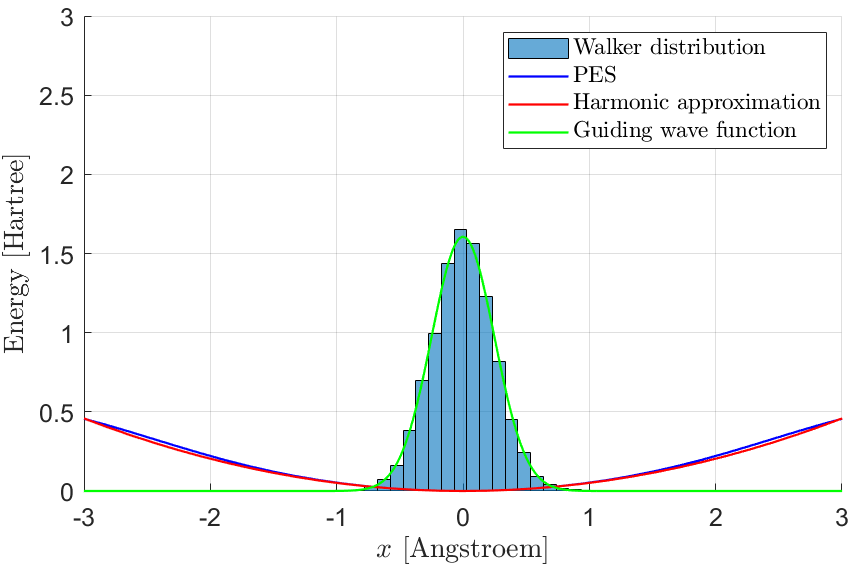
\includegraphics[width=0.9\linewidth, height=6cm]{walkers1.png} 
\caption{Dimension 7}
\label{dim7}
\end{subfigure}
\begin{subfigure}{0.5\textwidth}
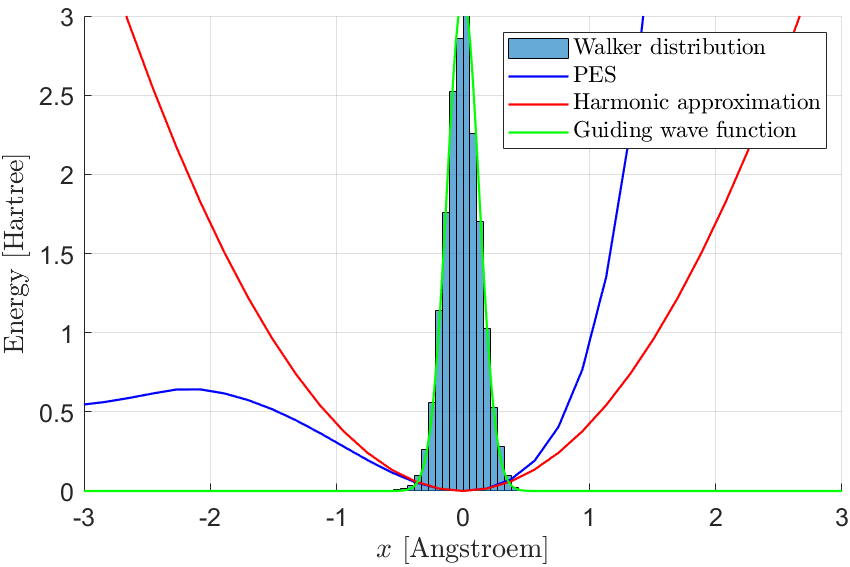
\includegraphics[width=0.9\linewidth, height=6cm]{walkers2.png}
\caption{Dimension 16}
\label{dim16}
\end{subfigure}
\caption{Comparison between the PES and the harmonic approximation for two example dimensions shows a good agreement up to the desired region of the harmonic approximation ZPE. The calculated trial wave function and the final distribution of the walkers also show excellent agreement.}
\label{trialwf}
\end{figure}
Next, we can check the harmonic approximation by comparing it to the true PES and calculate the trial wave function. For the ethane molecule, the harmonic approximation gives a ZPE of $0.072641$ Hartee. Therefore, we need the harmonic approximation to be good at least up to that value. With the trial wave function calculated, we can start the main calculation of the ZPE. We start with 10 parallel simulations of 1000 walkers and simulate for 10000 time steps of size $\Delta \tau = 5i \cdot 10^{-4}$. After the simulation, we can check if the walkers are distributed according to the trial wave function. Because the harmonic approximation is very good in this example, we expect the distribution of walkers to match the trial wave function.

\begin{appendices}
\chapter{The Box-Muller Algorithm} \label{appendixA}
The Box-Muller algorithm transforms two $\mathcal{U}([0,1])$ random numbers ($u_1, u_2$) to two $\mathcal{N}(0,1)$ random numbers ($x_1, x_2$).

\begin{algorithm}
\caption{Box-Muller Algorithm}\label{box-muller}
\begin{algorithmic}[1]
\Procedure{BoxMuller}{$u_1, u_2$}
\State $x_1 = sqrt(-2\log(u_1))\cos(2\pi u_2)$
\State $x_2 = sqrt(-2\log(u_1))\sin(2\pi u_2)$
\EndProcedure
\end{algorithmic}
\end{algorithm}

\chapter{The Metropolis Algorithm} \label{appendixB}
The Metropolis algorithm generates random numbers distributed according to a (high-dimensional) probability distribution $p(\bm{x})$ using a Markov Chain. A Metropolis step generates a new random number $\bm{x}_{i+1}$ from a given $\bm{x}_i$ that follows the probability distribution $p(\bm{x})$. It can also be used as the accept-reject step after the move of a walker. In this case, $f$ describes the propagation of the walker according to \eqref{2.10} and $\alpha$ becomes the acceptance probability \eqref{Pacc}.

\begin{algorithm}
\caption{Metropolis Step}\label{metropolis}
\begin{algorithmic}[1]
\Procedure{Metropolis}{$\bm{x}_i$}
\State $\bm{x}' = f(\bm{x}_i,$"noise"$)$ \Comment{proposing a new random number}
\State $\alpha = \frac{p(\bm{x}')}{p(\bm{x}_i)}$
\If{$\alpha \geq 1$}
	\State $\bm{x}_{i+1} = \bm{x}'$ \Comment{Accepting the proposed number}
\Else
	\State \textbf{draw} $u \sim \mathcal{U}([0,1])$
	\If{$u < \alpha$}
		\State $\bm{x}_{i+1} = \bm{x}'$ \Comment{Accepting the proposed number}
	\Else
		\State $\bm{x}_{i+1} = \bm{x}_i$ \Comment{Rejecting the proposed number}
	\EndIf
\EndIf 
\EndProcedure
\end{algorithmic}
\end{algorithm}

\chapter{Numerical Derrivatives for $E_L(x)$ and $v(x)$} \label{appendixC}
For a trial wave function $\psi(\bm{x})$ the first derivative used for the drift velocity $\bm{v}(\bm{x})$ is given by
\begin{equation}
\psi'(x) \approx \frac{\psi(x + h) - \psi(x - h)}{2h},
\end{equation}
and the second derivative used for the local energy $E_L(\bm{x})$ is given by
\begin{equation}
\psi''(x) \approx \frac{\psi(x + h) - 2 \psi(x) + \psi(x - h)}{h^2},
\end{equation}
where $h$ has to be chosen sufficiently small.

\chapter{Gradient Descent} \label{gradient_descent}
The gradient descent algorithm takes an input configuration $\bm{x}$ with the forces $\bm{f}$ and optimizes it with respect to the minimal energy $E_{min}$. There is a lot of freedom in the choice of the parameters that we will not discuss here. The here given algorithm gives some reasonable choices for the parameters. The idea of the gradient descent is to move along the negative gradient or forces to a region where the forces and the energy are lower. The step size $\alpha$ is adjusted depending on the angle between the current forces and the previous iteration. This way the step size increases if we have consecutive moves in the same direction and decreases if we start moving in an opposite direction. 
\begin{algorithm}
\caption{Gradient Descent}\label{grad_desc}
\begin{algorithmic}[1]
\Procedure{GradientDescent}{$\bm{x}, \bm{f}, E_{min}$} \Comment{calculate the energy and forces of a given configuration}
\State $\alpha = 10^{-3}$
\State call energyandforces($\bm{x}, \bm{f}, E_{min}$)
\While{$(||\bm{f}||/N_{at} > 10^{-6})$} \Comment{iterate up to a desired precision}
	\State $\bm{f}_{prev} = \bm{f}$	
	\State $\bm{x} = \bm{x} + \alpha \bm{f}$
	\State call energyandforces($\bm{x}, \bm{f}, E_{min}$)
	\State $\beta = \arccos{(<\bm{f},\bm{f_{prev}}>/\sqrt{||\bm{f}||\:||\bm{f}_{prev}||})}$ 
	\If{$(\beta/N_{at} > 1.0472)$} \Comment{60 degree in radians}
		\State $\alpha = \alpha/2$
	\Else
		\State $\alpha = 1.05\ \alpha$
	\EndIf
\EndWhile
\EndProcedure
\end{algorithmic}
\end{algorithm}
\end{appendices}

\bibliographystyle{unsrt}
\bibliography{references}

\end{document}